\documentclass[fontsize=11pt]{article}
\usepackage{lmodern}
\usepackage[protrusion=true,expansion=true]{microtype}
\usepackage[svgnames]{xcolor}  % Colours by their 'svgnames'
\usepackage[margin=0.75in]{geometry}
\textheight=700px
\usepackage{url}
\usepackage{lmodern} % Allow arbitrary font sizes
\usepackage{textcomp}

\usepackage{amssymb}
\usepackage{fontawesome5}
\usepackage{hyperref}
\hypersetup{
    colorlinks=false,
    pdfborder={0 0 0},
}

\usepackage{graphicx}

\usepackage[utf8]{inputenc}
\usepackage[T2A]{fontenc}
\usepackage[english,russian]{babel}

%% Define a new 'modern' style for the url package that will use a smaller font.
\makeatletter
\def\url@modernstyle{
  \@ifundefined{selectfont}{\def\UrlFont{\sf}}{\def\UrlFont{}}}
\makeatother
\urlstyle{modern} %% And use the newly defined style.

\frenchspacing              % Better looking spacings after periods
\pagestyle{empty}           % No pagenumbers/headers/footers

\renewcommand{\familydefault}{\sfdefault}

%%% Custom sectioning (sectsty package)
%%% ------------------------------------------------------------
\usepackage{sectsty}

\sectionfont{                 % Change font of \section command
  \sectionrule{0pt}{0pt}{-5pt}{3pt}}

%%% Macros
%%% ------------------------------------------------------------
\newlength{\spacebox}
\settowidth{\spacebox}{8888888888}      % Box to align text
\newcommand{\sepspace}{\vspace*{1em}}   % Vertical space macro

\newcommand{\MyName}[1]{ % Name
    \Huge \centering #1
    \par \normalsize \normalfont}

\newcommand{\NewPart}[1]{\section*{#1}}

\newcommand{\PersonalEntry}[2]{
    \noindent\hangindent=2em\hangafter=0 % Indentation
    \parbox{\spacebox}{                  % Box to align text
    \textit{#1}}                      % Entry name (birth, address, etc.)
    \hspace{1.5em} #2 \par}              % Entry value

\newcommand{\SkillsEntry}[2]{                % Same as \PersonalEntry
    \noindent\hangindent=2em\hangafter=0 % Indentation
    \parbox{\spacebox}{                  % Box to align text
    \textit{#1}}                    % Entry name (birth, address, etc.)
    \hspace{1.5em} #2 \par}              % Entry value

\newcommand{\AwardsEntry}[2]{                % Same as \PersonalEntry
    \noindent\hangindent=2em\hangafter=0 % Indentation
    \parbox{\spacebox}{                  % Box to align text
    \textit{#1}}                    % Entry name (birth, address, etc.)
    \hspace{1.5em} #2 \par}              % Entry value

\newcommand{\ProgrammingEntry}[2]{
    \noindent \textbf{#1} \hfill      % Study

    \noindent \small #2 % Description
    \normalsize \par}

\newcommand{\EducationEntry}[4]{
    \noindent \textbf{#1} \hfill      % Study
    \colorbox{Black}{
      \parbox{10em}{
      \color{White} \centering #2}} \par   % Duration
    \noindent \textit{#3} \par        % School
    \noindent\hangindent=2em\hangafter=0 \small #4 % Description
    \normalsize \par}

\newcommand{\WorkEntry}[3]{       % Same as \EducationEntry
    \noindent \large \textbf{#1} \hfill      % Jobname
    \colorbox{Black}{%
      \parbox{10em}{%
      \color{White} \centering #2}} \par  % Duration
    \noindent \small #3 % Description
    \normalsize \par}

\newcommand{\ProjectEntry}[4]{         % Similar to \EducationEntry
    \noindent \textbf{#1} \noindent \textit{#3} \hfill {#2} \par
    \noindent \small #4 % Description
    \normalsize \par}

\newcommand{\AwardEntry}[4]{         % Similar to \EducationEntry
    \noindent \textbf{#1} \noindent \textit{#3} \hfill {#2} \par
    \noindent \small #4 % Description
    \normalsize \par}
    \begin{document}



\begin{minipage}{0.2\textwidth}% adapt widths of minipages to your needs
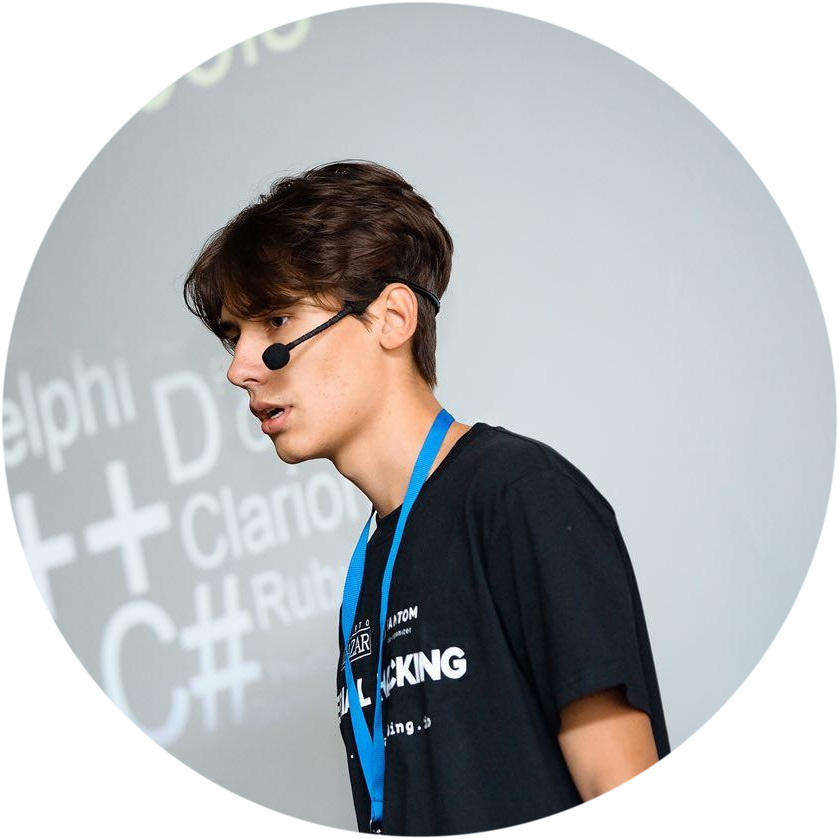
\includegraphics[width=4cm]{me.png}
\end{minipage}%
\hfill%
\begin{minipage}{14cm}\raggedright
\bigskip
\bigskip
\bigskip
\bigskip
\bigskip
\bigskip
\MyName{Dmitry Inyutin}
\bigskip
{inyutin.da@gmail.com | 89154336070 | \href{https://t.me/inyutin}{\faTelegram \, Telegram} | \href{https://github.com/inyutin}{\faGithub \, Github} | Москва}
\end{minipage}


%%% Work experience
%%% ------------------------------------------------------------ц

%%%
%%% Education
%%% ------------------------------------------------------------
\NewPart{Education}{}
\EducationEntry
{Bachelor in Applied Mathematics and Computer Science}
{2016 - 2020}
{Moscow Institute of Physics and Technology, Department of Innovation and High Technologies.}

\NewPart{Work experience}{}
\WorkEntry
{Assistant at MIPT}
{Spring 2019}
{I help on the course "Theory and Practice of Concurrent Computing". \\ I check students' homeworks and explain misunderstood at seminars and lectures.}

\bigskip

\WorkEntry
{Intern at Jetbrains}
{Summer 2018}
{I worked on a new product — web-based data analysis environment. \\ I made the online code editor more friendly and convenient for mobile devices.}

%%% Skills
%%% ------------------------------------------------------------
\NewPart{Knowledge of programming languages}{}
\ProgrammingEntry
{C++ \bigstar \bigstar \bigstar}
{I actively use ir for educational projects. \\ Familiar with standard containers and synchronization primitives.}
\bigskip
\ProgrammingEntry
{Python \bigstar \bigstar \bigstar}
{Constantly use for writing small programs, scripts.}
\bigskip
\ProgrammingEntry
{Java \bigstar \bigstar}
{I Worked with Java GWT and wrote a small backend on the Spring Framework. \\
Also I wrote several small Android apps.}
\bigskip
\ProgrammingEntry
{JavaScript \bigstar \bigstar}
{I Wrote a small server for blockchain application on NodeJs.}
\bigskip
\ProgrammingEntry
{Go \bigstar}
{I implemented a toy version of CASPaxos - Replicated State Machine without logs.}

\NewPart{Additional}{}
\SkillsEntry{Blockchain}{Worked with Ethereum API (web3js) and wrote applications using this technology.}
\SkillsEntry{Tools}{Git, Linux}

%%% Awards
%%% ------------------------------------------------------------
\NewPart{Participation in hackathons}{}

\AwardEntry{Cryptobazar, }{Winner}
{Moscow, September - December 2018}
{Various applications that somehow related to blockchain: pair encryption, \\ mobile crypto-wallet, virtual machine for WebAssembly.}
\sepspace
\AwardEntry{Phystech.Genesis,}{Winner}
{Moscow, September 2018}
{Android application for tourists, which finds interesting routes.}
\sepspace
\AwardEntry{Global Changers 2,}{Winner}
{Moscow, March 2018}
{Web service that creates interactive Customer Journey Maps.}
\sepspace
\AwardEntry{Birth.Hack,}{Participant}
{Moscow, April 2018}
{Web site where users can watch sports matches together using video chat.}
\sepspace
\AwardEntry{Global Changers 1,}{Winner}
{Moscow, March 2018}
{Video platform that encourages users for their social activity (uploading videos and comments).}
\sepspace
\AwardEntry{mABBYYlity,}{Participant}
{Moscow, October 2017}
{A small telegram-bot, which according to the photo of the barcode of the product shows customer\\ reviews and prices in the nearest stores.}

\NewPart{Projects}{}
\ProgrammingEntry
{ViBoard}
{A project that grew out of hackathon Global Changers 1. It was a video service where all the data was stored distributed on the IPFS network. We tried to build a community based economy. Every day there appeared a certain number of new coins, which were distributed to the most active users in a day. We supposed coins cost would be ensured by the popularity of the platform, but the project didn't took off.}
\bigskip
\ProgrammingEntry
{CASPaxos}
{CASPaxos is a distributed register without a log. \\ The main idea of CASPaxos is an attempt to replicate the state of the register, not the log. I wanted to figure out how it works and wrote my little implementation.}
\bigskip
\ProgrammingEntry
{MakeGood}
{A very small python script that cheers up by showing a positive and funny picture.}

\end{document}
